\documentclass{article}
\usepackage{../lambdatex} %disponibile all'indirizzo http://lambdamath.altervista.it/esercizi/lambdatex.sty
\usepackage{tasks}
\usepackage{exsheets}
\newcommand{\se}{\text{ se }}
\renewcommand{\phi}{\varphi}
\everymath{\displaystyle}

\title{Università degli Studi di Trento - Dipartimento di Matematica\\
CdL in Matematica – a.a. 2022–2023\\ Note esercitazione}
\author{Esercitatore: Simone Verzellesi\thanks{Trascrizione a cura di Davide Borra}}
\date{07 Dicembre 2022}
\begin{document}
\maketitle
\lhead{Note esercitazione}
\chead{Università degli Studi di Trento - Dipartimento di Matematica\\
CdL in Matematica – a.a. 2022–2023}
\rhead{07/12/2022}
\setlength{\headheight}{30pt}
% \begin{question}
%     pippo
%\end{question}
\begin{enumerate}[label=\textbf{Esercizio 11.\arabic*.},itemindent=*]
%%%%%%%%%%%%%%%%%%%%%%%%%%%%%%%%%%%%%%%%%%%%%%%%%%%%%
\item Siano $\beta\in \R$ e $S_\beta$ l'area del sottografico associato alla funzione $f(x)=x^2+\beta$ dove $x\in [-2,2]$.
\begin{tasks}
    \item disegnare la regione di piano $S_\beta$
    \item calcolare $S_\beta$
\end{tasks}
\item[\textit{\large Soluzione~}]~
Dobbiamo distinguere tre casi:
\begin{figure}[h]
    \centering
    \begin{subfigure}{0.27\textwidth}
        \centering
        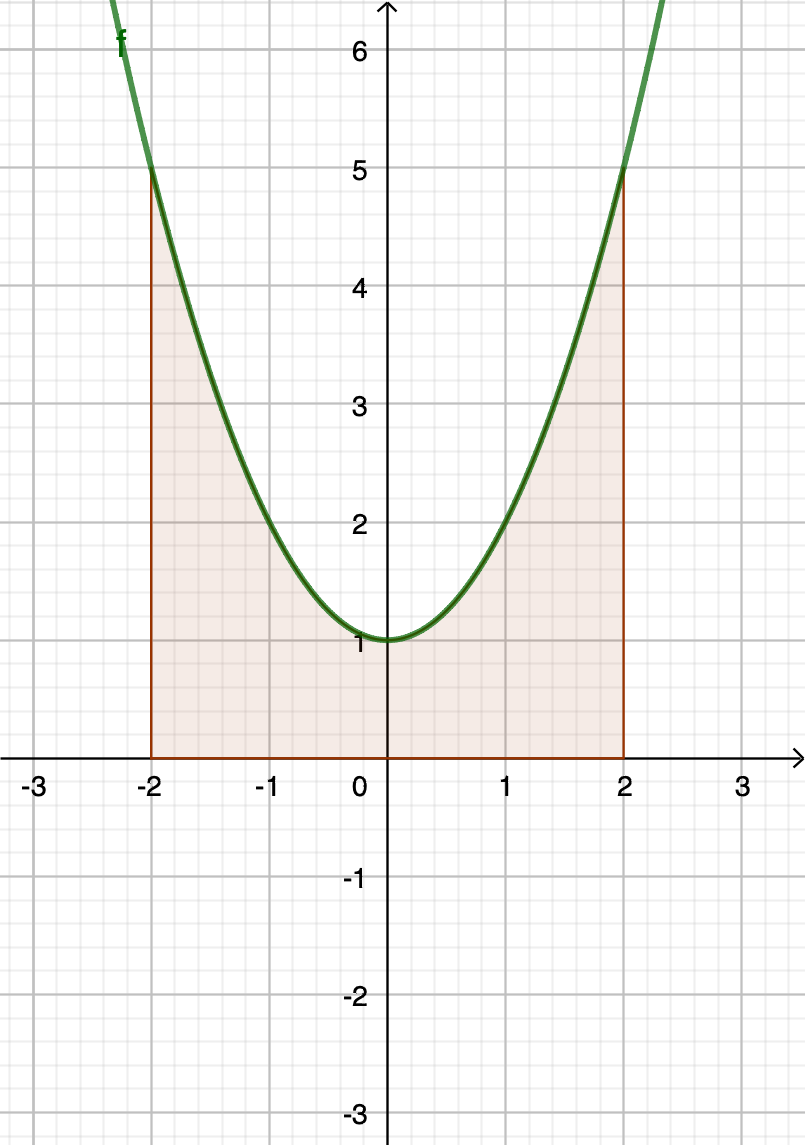
\includegraphics[width=.9\textwidth]{src/caso1.png}
        \caption{$\beta>0$}
        \label{subfig:caso1}
    \end{subfigure}
    \begin{subfigure}{0.27\textwidth}
        \centering
        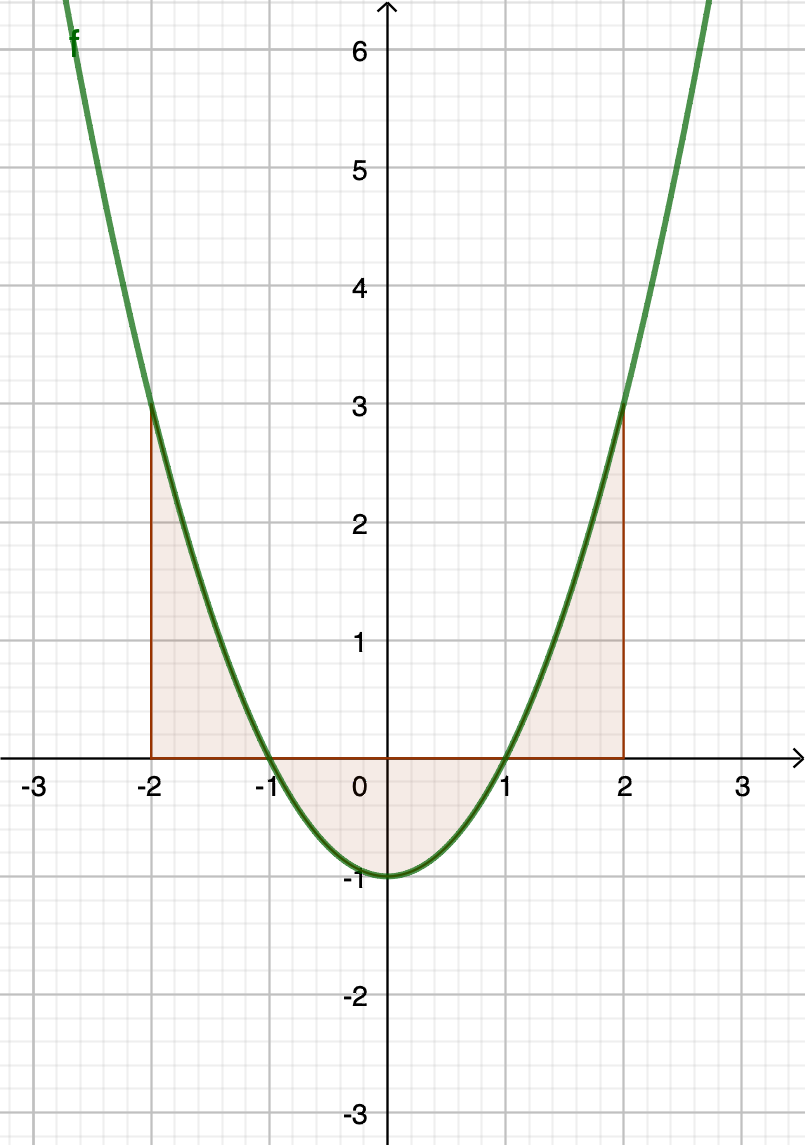
\includegraphics[width=0.9\textwidth]{src/caso2.png}
        \caption{$-4\leq\beta<0$}
        \label{fig:caso2}
    \end{subfigure}
    \begin{subfigure}{0.27\textwidth}
        \centering
        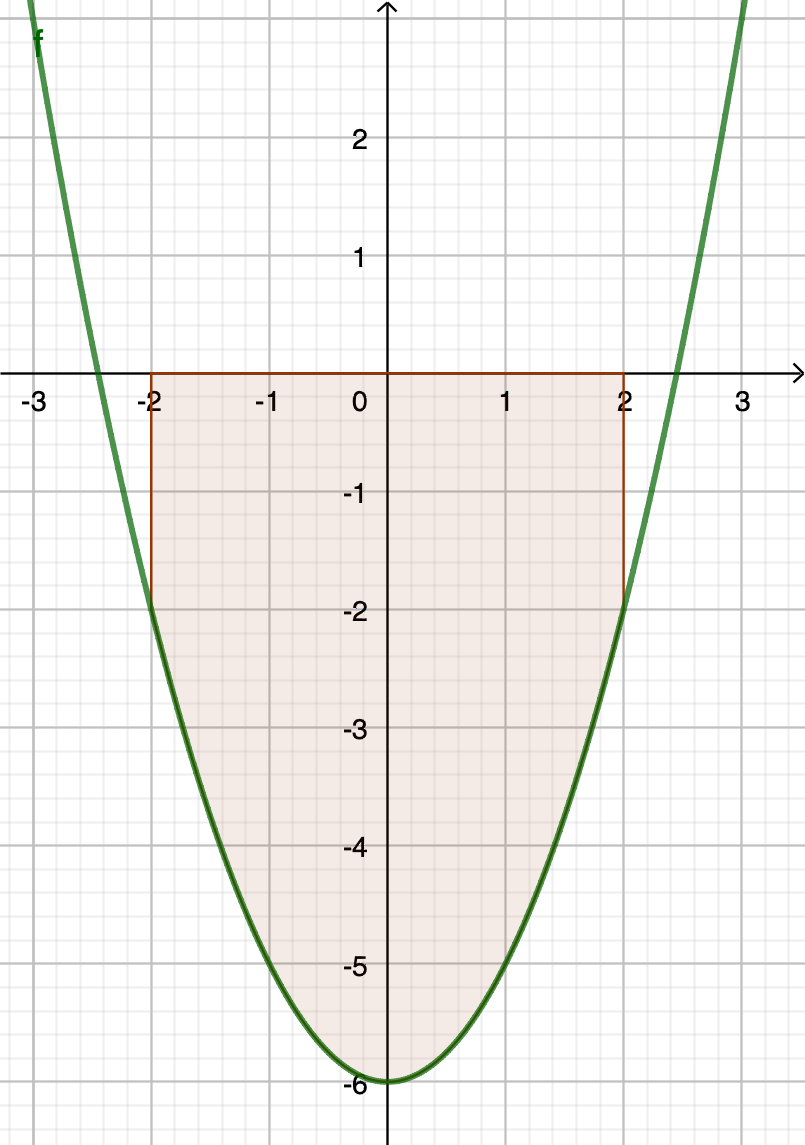
\includegraphics[width=.9\textwidth]{src/caso3.png}
        \caption{$\beta<-4$}
        \label{fig:caso3}
    \end{subfigure}
    \caption{}
\end{figure}
\begin{itemize}
    \item $\beta\geq0$ In questo caso la parabola si trova sempre sopra l'asse $x$ (Figura \ref{subfig:caso1}). \[S_\beta=\int_{-2}^2(x^2+\beta)dx\]
    \item Analizziamo ora quando la parabola interseca l'asse $x$ in due punti interni all'intervallo $[-2,2]$ (Figura \ref{fig:caso2})
    \[x^2+\beta=0~~\Harr~~x^2=-\beta~~\Harr~~x=\pm\sqrt{-\beta}\]
    \[\implies \exists x \in [-2,2]~:~f(x)=0~~\Harr -\beta\leq 4~~\Harr~~\beta\geq -4\]
    Di conseguenza, quando $-4\leq \beta<0$
    \[S_\beta=\int_{-2}^{2}|f(x)|dx=\int_{-2}^{-\sqrt{-\beta}}(x^2+\beta)dx+\int_{-\sqrt{-\beta}}^{\sqrt{-\beta}}(x^2+\beta)dx+\int_{\sqrt{-\beta}}^{2}(x^2+\beta)dx\]
    \item Rimane il caso in cui la parabola si trova sempre sotto l'asse $x$ in $[-2,2]$, ovvero quando $\beta<4$ (Figura \ref{fig:caso3}), in cui si ha
    \[S_\beta=-\int_{-2}^2(x^2+\beta)dx\]
\end{itemize}

%%%%%%%%%%%%%%%%%%%%%%%%%%%%%%%%%%%%%%%%%%%%%%%%%%%%%
\item Determinare l'area della regione di piano compresa tra $f(x)=\cos x$ e $g(x)=\sin x$ e le rette $x=0$ e $x=\pi$
\item[\textit{\large Soluzione~}]~
Prima di tutto determiniamo l'intersezione:
\[f(x)=g(x)~~\Harr~~x=\frac{\pi}{4}\]
\begin{figure}[h]
    \centering
    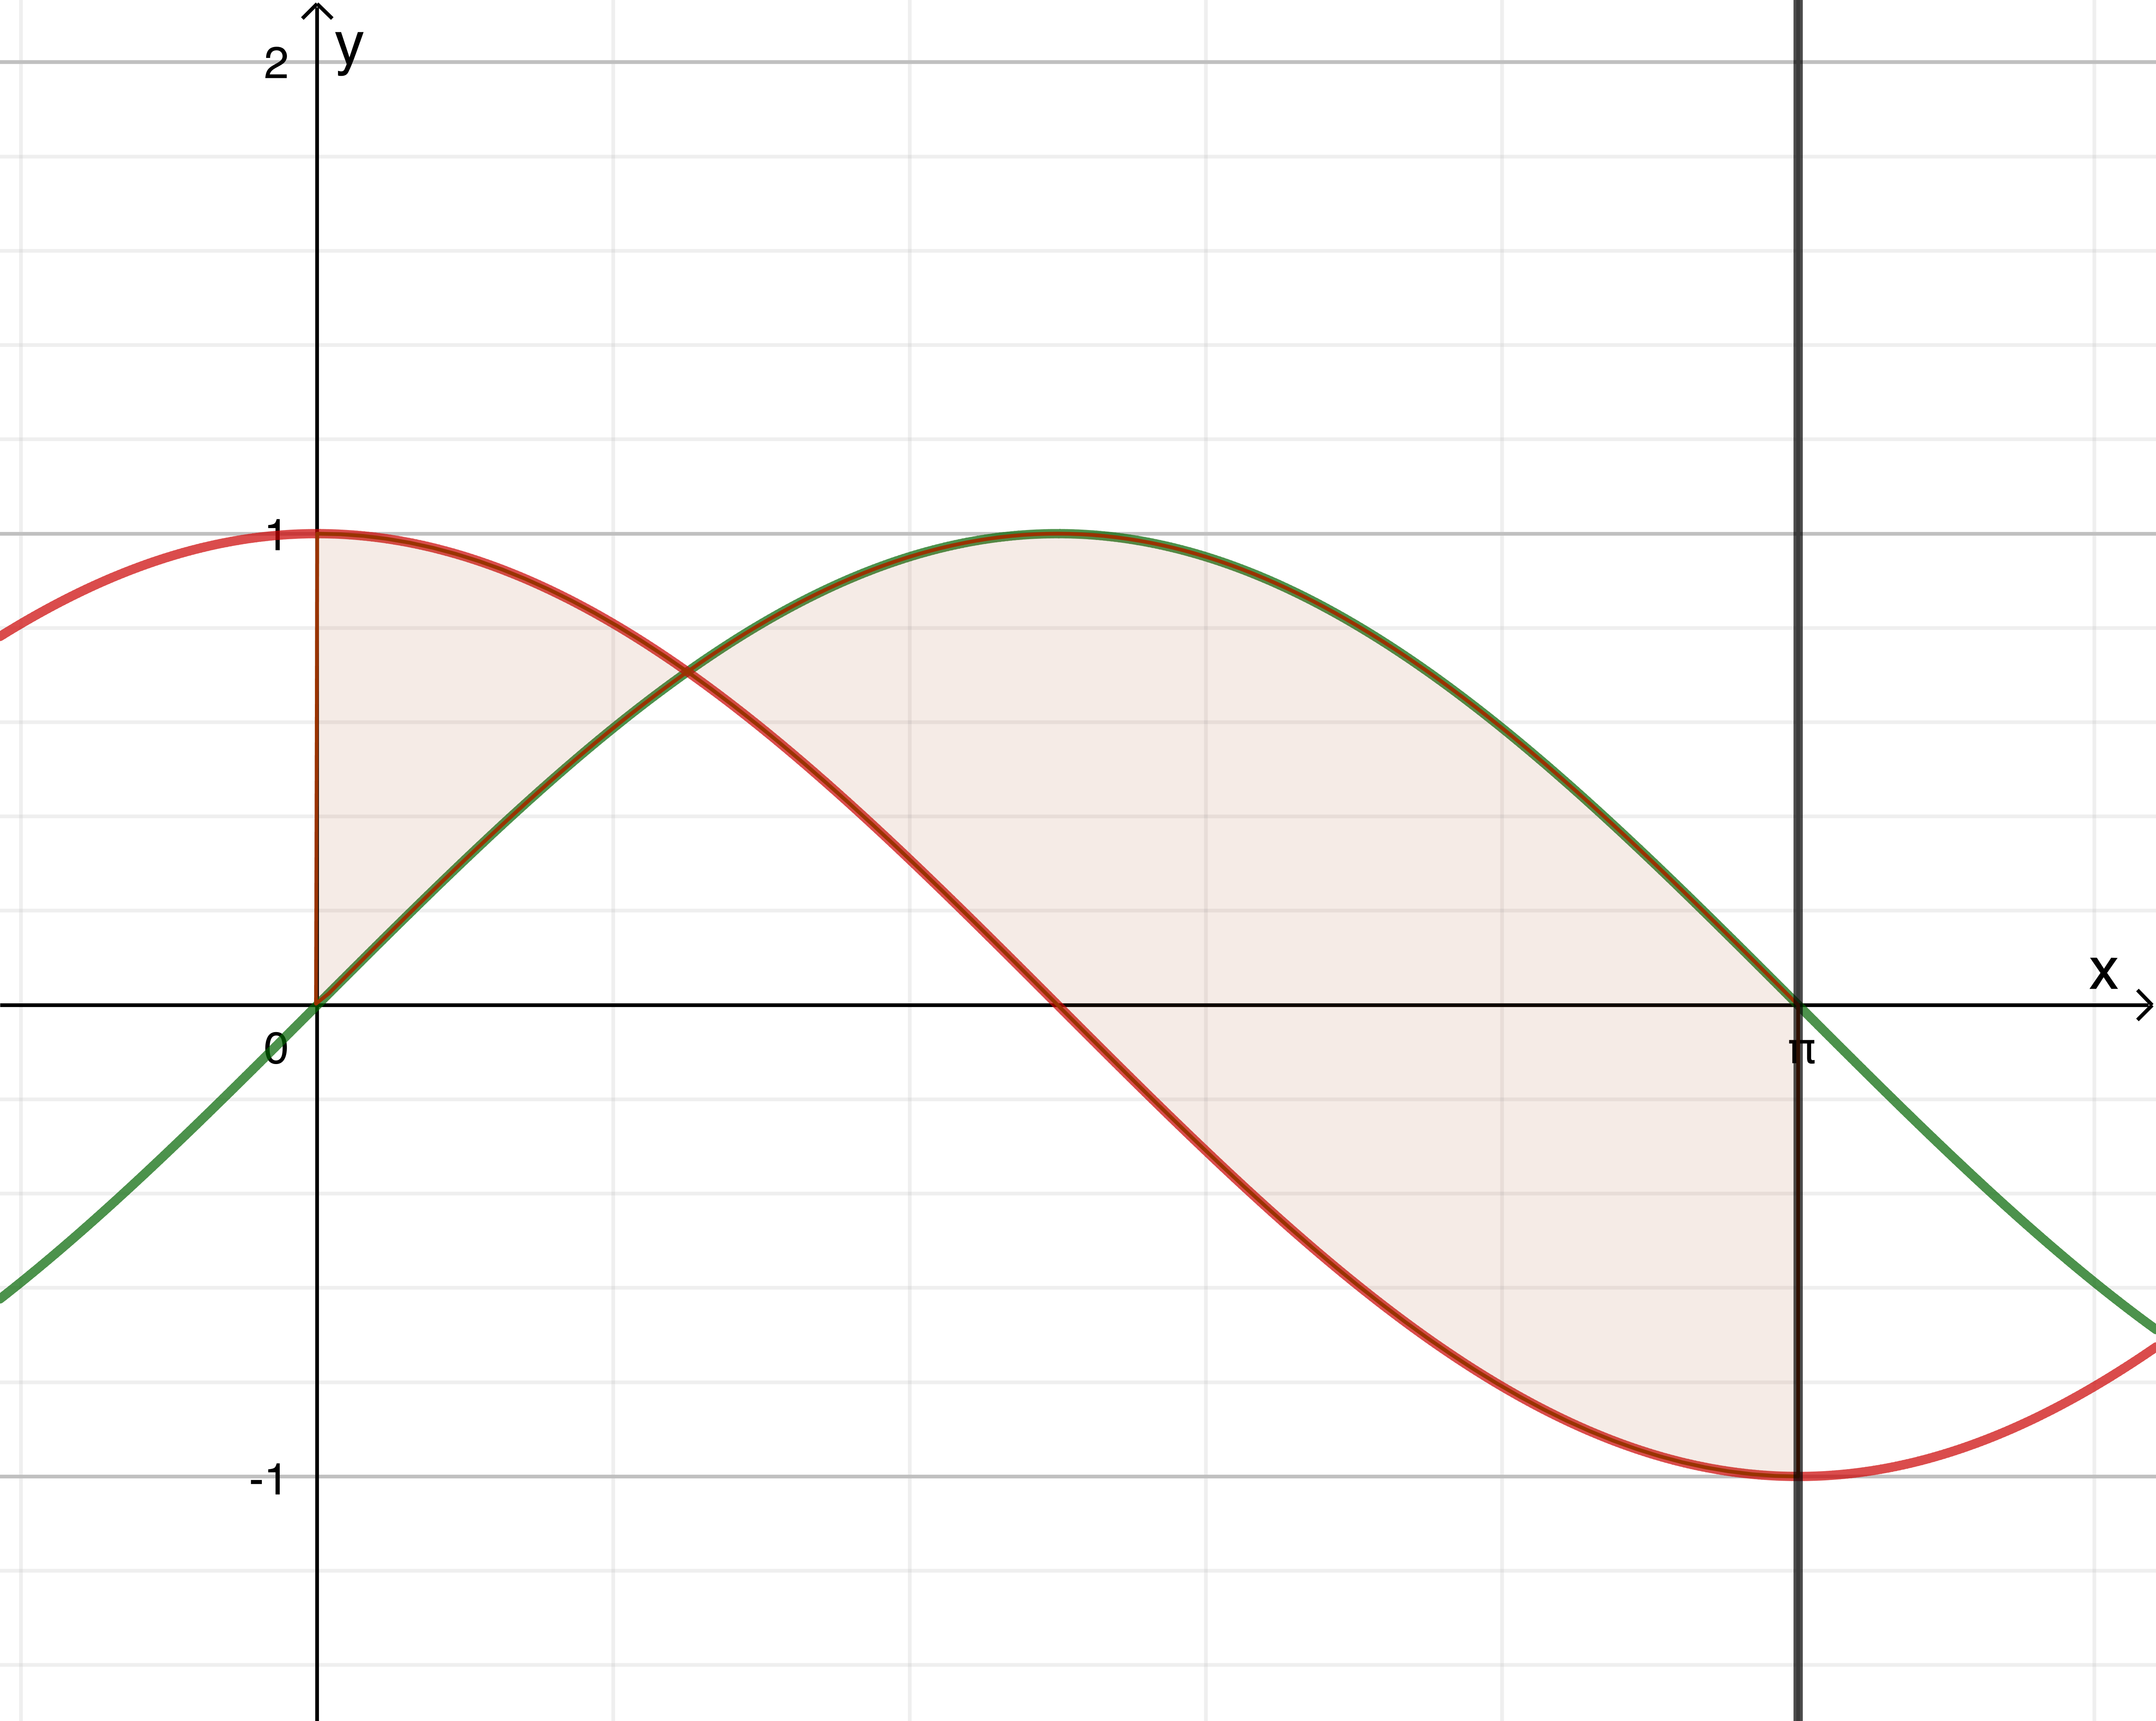
\includegraphics[width=0.5\textwidth]{src/es2.png}
    \caption{}
    \label{fig:es2}
\end{figure}
Abbiamo quindi che $f(x)\geq g(x)$ su $\left[ 0,\frac{\pi}{4} \right]$ e che $f(x)\leq g(x)$ su $\left[ \frac{\pi}{4} , \pi\right]$
Di conseguenza 
\[\begin{aligned}A&=\int _0^{\frac{\pi}{4}}(\cos x-\sin x)dx-\int_{\frac{\pi}{4}}^\pi(\cos x -\sin x)dx=[\sin x+\cos x]_0^{\frac{\pi}{4}}-[\sin x+\cos x]_{\frac{\pi}{4}}^\pi=\\ &=\left(\frac{\sqrt{2}}{2}+\frac{\sqrt{2}}{2}-0-1\right)-\left(\frac{0-1-\sqrt{2}}{2}-\frac{\sqrt{2}}{2}\right)=2\sqrt{2}\end{aligned}\]
%%%%%%%%%%%%%%%%%%%%%%%%%%%%%%%%%%%%%%%%%%%%%%%%%%%%%
\item Calcolare i seguenti integrali
\begin{tasks}(4)
    \task \(\int_{1}^{2}\frac{x+2\sqrt[3]{x}}{x^2}dx\)
    \task \(\int_{9}^{16}\frac{\sqrt{x}-3}{x-3\sqrt{x}+2}dx\)
    \task \(\int_{0}^{e-\frac{1}{e}}\sqrt{4-x^2}dx\)
    \task \(\int\frac{1}{1+\sin x}dx\)
\end{tasks}
\item[\textit{\large Soluzione~}]~
%%%%%%%%%%%%%%%%%%%%%%%%%%%%%%%%%%%%%%%%%%%%%%%%%%%%%

\end{enumerate}
\end{document}
